\osoba{Karol Liszka}

\section{Zadanie projektowe}			
\begin{itemize}	
	\item  
	\textbf{Rodzaj zadania:}   \hspace{1.5cm}  Przygotowanie środowiska programistycznego. C\#. \\
	\textbf{Data rozpoczęcia:} \hspace{1.0cm} 2015.10.20\\
	\textbf{Data zakończenia:} \hspace{0.95cm} 2015.10.22\\
	\textbf{Aktualny status:}  \hspace{1.25cm}  Zakończone\\
	
	\item  
	\textbf{Rodzaj zadania:}   \hspace{1.3cm}  Tworzenie programu. \\
	\textbf{Data rozpoczęcia:} \hspace{1.0cm} 2015.10.22\\
	\textbf{Data zakończenia:} \hspace{0.95cm} 2015.11.15\\
	\textbf{Aktualny status:}  \hspace{1.25cm}  Zakończone\\
	
		\item  
		\textbf{Rodzaj zadania:}   \hspace{1.3cm}  Poprawki do programu. \\
		\textbf{Data rozpoczęcia:} \hspace{1.0cm} 2015.11.17\\
		\textbf{Data zakończenia:} \hspace{0.95cm} 2015.12.01\\
		\textbf{Aktualny status:}  \hspace{1.25cm}  Zakończone\\
\end{itemize}

\section{Etapy budowania programu}
		
\subsection{Projektowanie formy}
Projekt budowania programu rozpoczął się od zaprojektowania okna z którym będzie miał styczność użytkownik. Okno jest jedynym elementem który użytkownik zobaczy, dla tego bardzo ważne jest aby było zrozumiałe i czytelne.\\
Poniżej okno programu:\\	
\begin{figure}
	\centering
	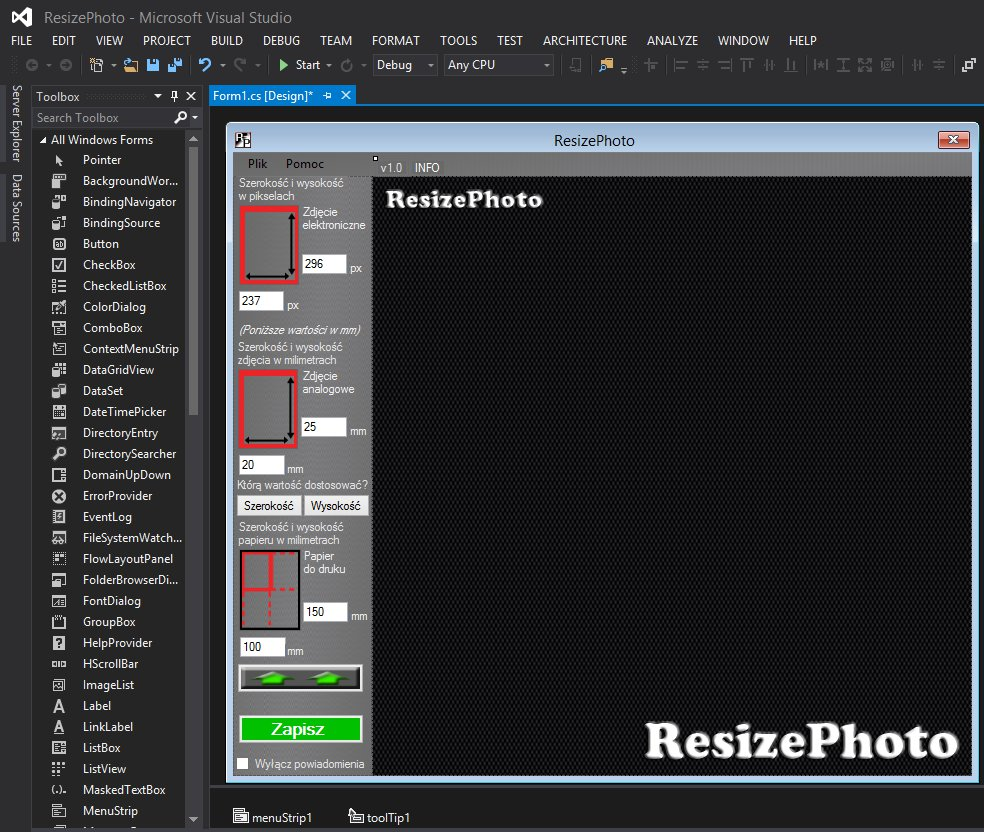
\includegraphics[width=12cm]{5.jpg}
	\caption{Okno aplikacji}
\end{figure} 

\lstset{xleftmargin=-3.5cm}
\subsection{Pisanie głównych funkcjonalności programu w języku C\#}
\begin{itemize}
\item \textbf{Funkcjonalność pól tekstowych. Pobieranie rozmiarów wyjściowych grafik. (textBox)}\\
\begin{lstlisting}
	
	 private void TextSzer1_TextChanged(object sender, EventArgs e)
	 {
	 bool result1 = Int32.TryParse(TextSzer1.Text, out SzerPiks);
	 if (result1)
	 {
	 TextSzer1.ForeColor = Color.Green;
	 SzerPiks = Int32.Parse(TextSzer1.Text);
	 bool result2 = Int32.TryParse(TextWys1.Text, out WysPiks);
	 if (result2)
	 {
	 WysPiks = Int32.Parse(TextWys1.Text);
	 }
	 else TextWys1.Text = "0";
	 SzerZdj = SzerPiks;
	 SzerPiksOld = SzerPiks;
	 WysPiksOld = WysPiks;
	 konwert = true;
	 
	 stosunekWH = (float)SzerPiks / (float)WysPiks;
	 
	 /*SzerMM = 0;
	 WysMM = 0;
	 TextWys2.Text = WysMM.ToString();
	 TextSzer2.Text = SzerMM.ToString();*/
	 
	 pictureBox1.Refresh();
	 if (SzerPiks > 0 && WysPiks> 0 && loaded)
	 {
	 WcisnietyX = 10;                                                                                        
	 WcisnietyY = 10;                                                                                        
	 Graphics g = pictureBox1.CreateGraphics();
	 Graphics g2 = pictureBox1.CreateGraphics();
	 Pen pen = new Pen(Color.Red, 2);
	 Pen pen2 = new Pen(Color.Yellow, 1);
	 
	 
	 
	 MainRect.X = 10;
	 MainRect.Y = 10;
	 
	 if (SzerPiksOld <= 550 && WysPiksOld <= 550)                                                           
	 {
	 MainRect.Width = (int)SzerPiksOld;
	 MainRect.Height = (int)WysPiksOld;
	 }
	 else if (SzerPiksOld > 550 || WysPiksOld > 550 && 
	 (SzerPiksOld < 1100 && WysPiksOld < 1100))
	 {
	 MainRect.Width = (int)(SzerPiksOld / 2);
	 MainRect.Height = (int)(WysPiksOld / 2);
	 }
	 else if (SzerPiksOld > 1100 || WysPiksOld > 1100)
	 {
	 MainRect.Width = (int)(SzerPiksOld / 4);
	 MainRect.Height = (int)(WysPiksOld / 4);
	 }                                                                                              
	 
	 pictureBox1.Refresh();
	 g.DrawRectangle(pen, MainRect);
	 
	 
	 
	 MiniRect.X = MainRect.X + MainRect.Width - 6;
	 MiniRect.Y = MainRect.Y + MainRect.Height - 6;
	 MiniRect.Width = 6;
	 MiniRect.Height = 6;
	 
	 
	 SolidBrush brush1 = new System.Drawing.SolidBrush
	 (System.Drawing.Color.Yellow);
	 g2.FillRectangle(brush1, MiniRect);
	 brush1.Dispose();
	 pen.Dispose();
	 g.Dispose();
	 g2.Dispose();
	 pen2.Dispose();
	 
	 
	 }
	 
	 }
	 else
	 {
	 TextSzer1.ForeColor = Color.Red;
	 konwert = false;
	 }
	 labelInfo.Text =
	 "RZ:"+RealW.ToString()+"x"+RealH.ToString()+"|"+
	 "RZE:"+MainRect.Width.ToString()+"x"+MainRect.Height.ToString()+" "+
	 "PB:"+pictureBox1.Width.ToString()+"x"+pictureBox1.Height.ToString() +"|"+
	 "KOMP:"+pictureBox5.Width.ToString()+"x"+pictureBox5.Height.ToString()+"|"+
	 "RATIO:"+stosunekWH.ToString();
	 }
	 
	\end{lstlisting}
Powyższy kod służy do odczytywania w polu tekstowym od użytkownika Szerokości zdjęcia cyfrowego podawanej w pikselach. Na początku kod sprawdza czy wartość podana przez użytkownika jest cyfrą, następnie jeśli tak wykonuje szereg operacji przypisania tej wartości do odpowiednich zmiennych w celu wykorzystania ich w dalszej częsci kodu. Następnie odświeża obszar gdzie wyświetlana jest grafika, w celu narysowania nowego prostokąta do wycinania zdjęcia. Pozostała część kodu to kosmetyczne ulepszenia, jak przykładowo zmniejszenie prostokąta do wycinania, jeśli jego rozmiar jest większy niż rozmiar okna aplikacji, tak aby zmieścił się w oknie. Na samym końcu aktualizujemy pasek stanu o zedytowane wartości//
Pozostale pola tekstowe są zbudowane bardzo podobnie z małymi zmianami zależnymi od tego jakie informacje przyjmują.
\end{itemize}

\begin{itemize}
\item \textbf{Załadowanie grafiki do programu.}\\
\begin{lstlisting}
	
	   private void LoadPhoto(object sender, EventArgs e)
	   {
	   OpenFileDialog ofd = new OpenFileDialog();
	   ofd.Filter = "jpg(*.jpg)|*.jpg|bmp (*.bmp)|*.bmp|
	   png (*.png)|*.png|gif (*.gif)|*.gif";
	   
	   if (ofd.ShowDialog() == DialogResult.OK && ofd.FileName.Length > 0)
	   {
	   pictureBox1.SizeMode = PictureBoxSizeMode.Zoom;
	   zaladowaneZdj = Image.FromFile(ofd.FileName);
	   pictureBox1.Image = zaladowaneZdj;
	   loaded = true;
	   RealW = zaladowaneZdj.Width;
	   RealH = zaladowaneZdj.Height;
	   }
	   
	   labelInfo.Text =
	   "RZ:"+RealW.ToString()+"x"+RealH.ToString()+"|"+
	   "RZE:"+MainRect.Width.ToString()+"x"+MainRect.Height.ToString()+" "+
	   "PB:"+pictureBox1.Width.ToString()+"x"+pictureBox1.Height.ToString() +"|"+
	   "KOMP:"+pictureBox5.Width.ToString()+"x"+pictureBox5.Height.ToString()+"|"+
	   "RATIO:"+stosunekWH.ToString();
	   
	   #region SKALOWANIE DO ROZMIARU ZDJECIA
	   
	   if (RealW > RealH)
	   {
	   int i;
	   this.Height = 600+63;
	   i= (int)((zaladowaneZdj.Width * 600) / zaladowaneZdj.Height);
	   this.Width = i+155;               
	   this.FormBorderStyle = System.Windows.Forms.FormBorderStyle.FixedSingle;
	   firstklik = true;
	   }
	   else if (RealW < RealH)
	   {
	   int i;
	   this.Height = 600+63;  
	   i= (int)((zaladowaneZdj.Width * 600) / zaladowaneZdj.Height);
	   this.Width = i+155;             
	   this.FormBorderStyle = System.Windows.Forms.FormBorderStyle.FixedSingle;
	   firstklik = true;
	   }
	   else 
	   {
	   this.Height = 600 + 63;
	   this.Width = 600 + 155;
	   this.FormBorderStyle = System.Windows.Forms.FormBorderStyle.FixedSingle;
	   firstklik = true;
	   }
	   #endregion
	   
	\end{lstlisting}
	
Powyższa część kodu odpowiada za przycisk do wczytywania zdjęć i ładowania do obiektu zwanego pictureBox.
Na początku kodu otwieramy okno dialogowe ustalając rozszerzenie plików możliwych do wczytania (w obecnym przypadku konieczne jest ustawienie filtru na pliki graficzne z rozszerzeniem takim jak bmp, jpg, png czy gif). Następnie kod ładuje wybrana grafikę do pictureBox pobierając przy tym jej prawdziwy wymiar. Na końcu kod aktualizuje pasek stanu o zmienione wartości oraz skaluje rozmiar okna odpowiednio do grafiki tak aby wypełniała ona całego pictureBox'a. Dodatkowo w kodzie został stworzony blok kodu za pomocą słowa kluczowego \#region i \#endregion. Jest to część typowo kosmetyczna ułatwiająca odczyt i edycję kodu.	
\end{itemize}
 
\begin{itemize}
	\item \textbf{Rysowanie prostokąta do wycinania grafiki (Rectangle)}\\
\begin{lstlisting}
	 private void pictureBox1_MouseMove(object sender, MouseEventArgs e)
	 {
	 currentPosMove.X = e.X;
	 currentPosMove.Y = e.Y;
	 if (MiniRect.Contains(currentPosMove) | skalowanie)
	 Cursor = Cursors.SizeNWSE;
	 else if (MiniRect.Contains(currentPosMove) == false &&
	 (MainRect.Contains(currentPosMove) | przeciaganie))
	 Cursor = Cursors.Hand;
	 else
	 Cursor = Cursors.Default;
	 
	 Graphics g = pictureBox1.CreateGraphics();
	 Graphics g2= pictureBox1.CreateGraphics();
	 Pen pen = new Pen(Color.Red, 2);
	 Pen pen2 = new Pen(Color.Yellow, 1);
	 labelInfo.Text =
	 "RZ:"+RealW.ToString()+"x"+RealH.ToString()+"|"+
	 "RZE:"+MainRect.Width.ToString()+"x"+MainRect.Height.ToString()+" "+
	 "PB:"+pictureBox1.Width.ToString()+"x"+pictureBox1.Height.ToString() +"|"+
	 "KOMP:"+pictureBox5.Width.ToString()+"x"+pictureBox5.Height.ToString()+"|"+
	 "RATIO:"+stosunekWH.ToString();
	 
	 if ((firstklik||isDown) && (przeciaganie || firstklik)
	  && SzerPiks > 0 && WysPiks > 0&&loaded)
	 {
	 
	 korner[0].X = e.X - (WcisnietyX - oldX);
	 korner[0].Y = e.Y - (WcisnietyY- oldY);
	 
	 korner[1].X = e.X + ((WcisnietyX - oldX) + MainRect.Width);
	 korner[1].Y = e.Y - (WcisnietyY - oldY);
	 
	 korner[2].X = e.X + ((WcisnietyX - oldX) + MainRect.Width);
	 korner[2].Y = e.Y + ((WcisnietyY - oldY) + MainRect.Height);
	 pictureBox1.Refresh();

	 korner[2].Y - korner[1].Y);
	 MainRect.X = e.X - (WcisnietyX - oldX);
	 MainRect.Y = e.Y - (WcisnietyY - oldY);
	 if (SzerPiksOld <= 550 && WysPiksOld <= 550)                                                           
	 {
	 MainRect.Width = SzerPiks;
	 MainRect.Height = WysPiks;
	 }
	 else if (SzerPiksOld > 550 || WysPiksOld > 550 &&
	 (SzerPiksOld < 1100 && WysPiksOld < 1100))
	 {
	 MainRect.Width = SzerPiks / 2;
	 MainRect.Height = WysPiks / 2;
	 }
	 else if (SzerPiksOld > 1100 || WysPiksOld > 1100)
	 {
	 MainRect.Width = SzerPiks / 4;
	 MainRect.Height = WysPiks / 4;
	 }                                                                                              
	 g.DrawRectangle(pen, MainRect);
	 
	
	 PozX = korner[1].X - korner[0].X;
	 PozY = korner[2].Y - korner[1].Y;
	 
	 MiniRect.X = MainRect.X + MainRect.Width - 6;
	 MiniRect.Y = MainRect.Y + MainRect.Height - 6;
	 MiniRect.Width = 6;
	 MiniRect.Height = 6;
	 SolidBrush brush1 = new System.Drawing.SolidBrush
	 (System.Drawing.Color.Yellow);
	 g2.FillRectangle(brush1, MiniRect);
	 MiniRect.Width = 10;
	 MiniRect.Height = 10;
	 brush1.Dispose();
	 
	 pen.Dispose();
	 g.Dispose();
	 g2.Dispose();
	 pen2.Dispose();
	 
	 }

	 if (isDown && skalowanie&&loaded)
	 {
 
	 pictureBox1.Refresh();
	 
	 MainRect.X = korner[0].X;
	 MainRect.Y = korner[0].Y;
	 if (SzerPiksOld <= 550 && WysPiksOld <= 550)                                                           
	 {
	 MainRect.Width = SzerPiks;
	 MainRect.Height = WysPiks;
	 }
	 else if (SzerPiksOld > 550 || WysPiksOld > 550 && 
	 (SzerPiksOld < 1100 && WysPiksOld < 1100))
	 {
	 MainRect.Width = SzerPiks / 2;
	 MainRect.Height = WysPiks / 2;
	 }
	 else if (SzerPiksOld > 1100 || WysPiksOld > 1100)
	 {
	 MainRect.Width = SzerPiks / 4;
	 MainRect.Height = WysPiks / 4;
	 }                                                                                              
	 g.DrawRectangle(pen, MainRect);
	 	 	 
	 if (e.X > PosW + 2 || e.Y > PosH + 2)
	 {
	 if (e.X > PosW + 2)
	 {
	 PosW = e.X;
	 SzerPiks += (int)(SzerPiksOld * 0.02);
	 PosH = e.Y;
	 WysPiks += (int)(WysPiksOld * 0.02);	 
	 }
	 if (e.Y > PosH + 2)
	 {
	 PosW = e.X;
	 SzerPiks += (int)(SzerPiksOld * 0.02);
	 PosH = e.Y;
	 WysPiks += (int)(WysPiksOld * 0.02);	 
	 }
	 }
	 else
	 {
	 if (e.X < PosW - 2)
	 {
	 PosW = e.X;
	 SzerPiks -= (int)(SzerPiksOld * 0.02);
	 PosH = e.Y;
	 WysPiks -= (int)(WysPiksOld * 0.02);	 
	 }
	 if (e.Y < PosH - 2)
	 {
	 PosW = e.X;
	 SzerPiks -= (int)(SzerPiksOld * 0.02);
	 PosH = e.Y;
	 WysPiks -= (int)(WysPiksOld * 0.02);	 
	 }
	 }	 
	 pen.Dispose();
	 g.Dispose();	 	 
	 }
	 }
	 
	\end{lstlisting}
	
Powyższy kod służy do rysowania czerwonego kwadratu (Rectangle) do wycinania kawałka grafiki, jednak podkreślam, że nie jest to jedyna funkcja która służy do rysowania rectangle. Zasługuje ona jednak na wyróżnienie ponieważ rysowanie rectangle głównie opiera się na tej funkcji.\\
Funkcja MouseMove odpowiada za poruszanie myszką w obiekcie pictureBox. Podczas wcisniętego prawego klawisza myszki poruszamy rectangle co oznacza ze cały czas jest rysowany na nowo w zaktualizowanych pozycjach, tak samo jest ze skalowaniem, tylko tutaj zamiast zmieniać pozycję zmieniamy rozmiar.	Piewsza instrukcja warunkowa if sprawdza pozycję kursora i w zalezności od niej ustawia wygląd kursora do jego obecnej funkcjonalności. Następnie w kodzie tworzymy nowe obiekty niezbędne do rysowania takie jak Pen. Dalej aktualizujemy pasek stanu o zaktualizowane wartości. Kolejna instrukcja warunkowa sprawdza czy grafika jest załadowana i czy użytkownik kliknął w odpowiednim miejscu aby przesunąć rectangle. Jeśli warunki są spełnione czerwony prostokąt z powodzeniem się przemieszcza. Jeszcze następna instrukcja warunkowa sprawdza czy kursor jest w prawy dolnym rogu rectangle i czy jest wciśnięty prawy przycisk myszy. Jeśli warunki są spełnione skalowanie czerwonego prostokąta do wycinania jest możliwe. 	Dodatkowo w tej funkcji wykonywane są różnorakie obliczenia polegające na dopasowaniu stosunku podanego przez użytkownika do narysowanego rectangle w programie bądź też obliczaniu odległości myszki od początku narysowanego rectangle w celu dogodnego przesuwania prostokąta bez względu na to gdzie klikniemy myszką (z wykluczeniem punktu do skalowania).\\
\end{itemize}


\begin{itemize}
\item \textbf{Wycinanie elementu wskazanego przez Rectangle}\\
\begin{lstlisting}
	 public Bitmap CropImage(Bitmap source, Rectangle section)
	 {
	 Bitmap bmp = new Bitmap(section.Width, section.Height);	
	 Graphics g = Graphics.FromImage(bmp);
	 g.DrawImage(source, 0, 0, section, GraphicsUnit.Pixel);	
	 return bmp;
	 } 

\end{lstlisting}
Powyższa funkcja wycina element grafiki znajdujący się wewnątrz narysowanego rectangle.Na początku funkcja tworzy nowy obiekt typu Bitmap, o wymiarach narysowanego przez użytkownika rectangle. następnie wypełnia ten obiekt elementem grafiki na który wskazuje rectangle poprzez swoją pozycję oraz rozmiar. Na końcu funkcja zwraca grafikę w postaci bitmapy.
\end{itemize}


\begin{itemize}
\item \textbf{Zapis grafiki do pliku z rozszerzeniem graficznym.}\\
\begin{lstlisting}
	private void SavePhotoToolStripMenuItem_Click(object sender, EventArgs e)
	{
	if (loaded)
	{
	SaveFileDialog sfd = new SaveFileDialog();
	sfd.Filter = "jpg (*.jpg)|*.jpg|bmp (*.bmp)|*.bmp| png(*.png)|*.png| 
	gif (*.gif)|*.gif";
	if (sfd.ShowDialog() == DialogResult.OK && sfd.FileName.Length > 0)
	{
	grafika=CropImage(new Bitmap(pictureBox1.Image, pictureBox1.Size),MainRect);
	Bitmap Crop1 = new Bitmap(grafika, new Size(SzerZdj, WysZdj));
	#region zapisywanie cyfrowego
	try
	{
	Crop1.SetResolution(72.0f, 72.0f);
	Crop1.Save(sfd.FileName, ImageFormat.Jpeg);
	if (!powiadomienia)
	{
	MessageBox.Show("Zdjecie cyfrowe zostalo zapisane.", "Zapis", 
	MessageBoxButtons.OK, MessageBoxIcon.Information);
	}}
	catch (Exception)
	{
	MessageBox.Show("Zmien nazwe zapisywanego pliku.", "Blad01", 
	MessageBoxButtons.OK, MessageBoxIcon.Error);
	}}}
	#endregion
	}     

\end{lstlisting}
Podobnie jak w poprzednich przykładach, również tutaj podam jedną z przykładowych funkcji które wchodzą w skład programu. Funkcje działaja bardzo podobnie, różniąc się głównie wymiarami grafik jakie mają zapisać.
Powyższa funkcja odpowiada za zapisanie pliku do zdjęcia cyfrowego(dwie pierwsze wartości podane w programie).
Na początku oczywiście otwiera okno dialogowe w celu wskazania miejsca zapisu pliku oraz nazwy jaką chcemy nadać. Dzięki filtrowi mamy pewność, że zapisany plik będzie miał rozszerzenie zgodne z oczekiwaniami.
Następnie jest wywoływana funkcja do wycinania grafiki. Wycięta grafika jest zapisywana do pliku za pomocą funkcji Save(). Jeśli zdjęcie zostało zapisane z powodzeniem, wyświeli się komunikat, jeśli jednak wystąpił błąd, program zwróci powiadomienie o błędzie i dodatkowo wyświeli wskazówkę jak ominąc błąd.
\end{itemize}
\subsection{Czego nauczyłem się indywidualnie}
\begin{itemize}
	\item Wykorzystywać obiekt pictureBox do przechowywania grafiki,
	\item Używać część możliwości biblioteki drawing,
	\item Za pomocą Rectangle wycinać elementy graficzne,
	\item Wyłapywać błędy w trakcie działania programu i zwracać komunikaty o nich,
	\item Tworzyć dokumentację tworzonego programu,
	\item Utrzymywać kod w ładzie i porządku aby był czytelny i łatwy do dalszej edycji,
	\item Dostosowywać się do potrzeb i wymagań zleceniodawcy.
\end{itemize}
\subsection{Czego nauczyłem się zespołowo}
\begin{itemize}
	\item Współpracować w zespole projektowym,
	\item Dotrzymywać terminów prowadzenia prac projektowych,
	\item Wykonywania zadan zleconych przez menadżera projektu.
\end{itemize} 